\section{Supplementary pooling, metrics, and uncertainty}
\label{sec:supplement}
The supplementary \meanmodel{} uses the same training seed 44, five-fold probability-ensemble rule, observed-history protocol, future-state objective, and forecast classifier feature groups as \fullmodel{}, replacing spatial attention with mean pooling. Its metrics are computed from patient-wise mean probabilities, consistent with the main analysis.
\begin{table*}[t]
\centering
\small
\caption{Supplementary pooling comparison using seed44 fivefold probability ensembles. ForecastMean and ForecastAttention share forecast readout and future-state supervision, differing in spatial pooling. Probabilities are averaged before metrics; Macro averages the three landmarks.}
\label{tab:pooling}
\begin{tabular}{llrrr}
\toprule
Model & Landmark & AUROC & AP & F1 \\
\midrule
ForecastMean & T0 & 0.7431 & 0.6088 & 0.5625 \\
ForecastMean & T1 & 0.7494 & 0.6121 & 0.5865 \\
ForecastMean & T2 & 0.7471 & 0.6209 & 0.5736 \\
ForecastMean & Macro & 0.7465 & 0.6139 & 0.5742 \\
ForecastAttention & T0 & 0.7450 & 0.6256 & 0.5736 \\
ForecastAttention & T1 & 0.7521 & 0.6278 & 0.5442 \\
ForecastAttention & T2 & 0.7550 & 0.6315 & 0.5634 \\
ForecastAttention & Macro & 0.7507 & 0.6283 & 0.5604 \\
\bottomrule
\end{tabular}
\end{table*}

\begin{table*}[t]
\centering
\footnotesize
\setlength{\tabcolsep}{5pt}
\caption{All 14 macro metrics for the principal variants: point estimate [95\% patient-bootstrap percentile interval]. Each patient\textquotesingle s five seed44 fold-model probabilities are averaged first; metrics are then computed and equally averaged over T0--T2. Threshold-dependent metrics use 0.5. Identical patient resamples preserve pairing across models and landmarks. Entries are marginal model intervals; paired differences are reported separately. Intervals condition on the fitted ensembles and exclude retraining and retrospective selection uncertainty. Downward arrows identify metrics for which lower is better.}
\label{tab:extended_macro}
\begin{tabular}{lccc}
\toprule
Metric & NoJEPA & DirectReadout & ForecastAttention \\
\midrule
AUROC & 0.7279 [0.6501, 0.8046] & 0.7399 [0.6653, 0.8155] & 0.7507 [0.6741, 0.8268] \\
AP & 0.5968 [0.4703, 0.7141] & 0.6075 [0.4816, 0.7235] & 0.6283 [0.5066, 0.7465] \\
F1 & 0.5416 [0.4330, 0.6397] & 0.5678 [0.4626, 0.6612] & 0.5604 [0.4605, 0.6564] \\
Accuracy & 0.6648 [0.5980, 0.7334] & 0.6781 [0.6114, 0.7429] & 0.6495 [0.5829, 0.7181] \\
Sensitivity & 0.6190 [0.4909, 0.7487] & 0.6607 [0.5333, 0.7836] & 0.6964 [0.5723, 0.8187] \\
Specificity & 0.6863 [0.6043, 0.7667] & 0.6863 [0.6048, 0.7634] & 0.6275 [0.5478, 0.7057] \\
PPV & 0.4815 [0.3667, 0.5970] & 0.4981 [0.3892, 0.6117] & 0.4705 [0.3684, 0.5774] \\
NPV & 0.7929 [0.7130, 0.8695] & 0.8113 [0.7352, 0.8865] & 0.8145 [0.7347, 0.8917] \\
Balanced accuracy & 0.6527 [0.5759, 0.7268] & 0.6735 [0.6016, 0.7460] & 0.6619 [0.5930, 0.7360] \\
MCC & 0.2894 [0.1454, 0.4312] & 0.3277 [0.1906, 0.4617] & 0.3038 [0.1737, 0.4424] \\
Youden index & 0.3053 [0.1518, 0.4535] & 0.3470 [0.2031, 0.4919] & 0.3239 [0.1861, 0.4720] \\
NLL $\downarrow$ & 0.5822 [0.5192, 0.6442] & 0.5819 [0.5213, 0.6418] & 0.5990 [0.5613, 0.6364] \\
Brier score $\downarrow$ & 0.2010 [0.1739, 0.2279] & 0.2001 [0.1735, 0.2268] & 0.2061 [0.1883, 0.2235] \\
ECE $\downarrow$ & 0.1337 [0.0979, 0.2015] & 0.1272 [0.0901, 0.1964] & 0.1687 [0.1175, 0.2281] \\
\bottomrule
\end{tabular}
\end{table*}

\begin{table*}[t]
\centering
\small
\caption{Operating-point sensitivity analysis for seed-44 test ensemble scores, shown as three-landmark metric means. The alternative threshold maximizes Youden index on concatenated, disjoint out-of-fold development predictions, separately at each landmark; the largest threshold breaks ties. Each development patient contributes one score from a model that did not train on that patient. OOF scores arise from single fold models, whereas test scores average five model probabilities: this distribution mismatch makes this a sensitivity analysis, not validated ensemble calibration. No test labels select thresholds.}
\label{tab:extended_threshold}
\begin{tabular}{llrrrr}
\toprule
Model & Policy & F1 & Sens. & Spec. & MCC \\
\midrule
NoJEPA & 0.5 & 0.542 & 0.619 & 0.686 & 0.289 \\
NoJEPA & OOF validation Youden & 0.547 & 0.655 & 0.653 & 0.289 \\
\midrule
DirectReadout & 0.5 & 0.568 & 0.661 & 0.686 & 0.328 \\
DirectReadout & OOF validation Youden & 0.571 & 0.655 & 0.700 & 0.336 \\
\midrule
ForecastAttention & 0.5 & 0.560 & 0.696 & 0.627 & 0.304 \\
ForecastAttention & OOF validation Youden & 0.563 & 0.720 & 0.605 & 0.304 \\
\bottomrule
\end{tabular}
\end{table*}


\subsection{Paired significance checks}
Table~\ref{tab:bootstrap} combines the principal Macro comparisons with their unadjusted 95\% patient-bootstrap intervals, raw two-sided $p$ values, and Holm-adjusted $p$ values for the nine-test principal family. AUROC uses paired DeLong tests; other metrics use approximate null-centered paired patient-bootstrap tests with 99,999 shared patient resamples. The secondary family comprises 81 tests, reported in Tables~\ref{tab:significance_landmarks}--\ref{tab:significance_longitudinal}. These use the same seed-44 ensemble predictions and the same 175 patients, retaining model and landmark dependence. A significance marker refers to its stated Holm-adjusted family; ns denotes $p_{\mathrm{Holm}}\geq0.05$. The existing unadjusted 2,000-resample percentile intervals are not exact inversions of these tests and do not establish significance after correction. The original score-swap tests are retained separately in the source package: they test the stronger score-exchangeability null and do not determine these markers. The main testing method was revised after inspecting initial score-swap results; all tests and reporting choices remain retrospective and exploratory.

\begin{table*}[t]
\centering
\small
\caption{Exploratory landmark comparisons. AUROC uses paired DeLong tests; other metrics use approximate, null-centered paired patient-bootstrap tests (99,999 shared resamples). All $p$ values are two-sided. $p_{\mathrm{Holm}}$ adjusts jointly over the 81 secondary tests in Tables~\ref{tab:significance_landmarks}--\ref{tab:significance_longitudinal}. Direct and Attention abbreviate DirectReadout and ForecastAttention. $^{*}p_{\mathrm{Holm}}<0.05$, $^{**}p_{\mathrm{Holm}}<0.01$, $^{***}p_{\mathrm{Holm}}<0.001$; ns, not significant after the stated correction. Intervals are unadjusted 95\% patient-bootstrap intervals (2,000 shared draws) and need not agree with adjusted test decisions. All analyses condition on the fitted, retrospectively selected seed44 ensembles.}
\label{tab:significance_landmarks}
\begin{tabular}{lllrrrc}
\toprule
Comparison & Landmark & Metric & Difference [95\% CI] & $p$ & $p_{\mathrm{Holm}}$ & Sig. \\
\midrule
Direct -- NoJEPA & T0 & AUROC & +0.0098 [-0.0074, +0.0274] & 0.2414 & 1.0000 & ns \\
Direct -- NoJEPA & T0 & AP & +0.0071 [-0.0144, +0.0283] & 0.4821 & 1.0000 & ns \\
Direct -- NoJEPA & T0 & F1 & +0.0315 [+0.0000, +0.0722] & 0.0886 & 1.0000 & ns \\
Direct -- NoJEPA & T1 & AUROC & +0.0135 [-0.0032, +0.0312] & 0.1218 & 1.0000 & ns \\
Direct -- NoJEPA & T1 & AP & +0.0134 [-0.0111, +0.0397] & 0.2842 & 1.0000 & ns \\
Direct -- NoJEPA & T1 & F1 & +0.0266 [-0.0047, +0.0669] & 0.1543 & 1.0000 & ns \\
Direct -- NoJEPA & T2 & AUROC & +0.0129 [-0.0032, +0.0299] & 0.1233 & 1.0000 & ns \\
Direct -- NoJEPA & T2 & AP & +0.0115 [-0.0133, +0.0365] & 0.3588 & 1.0000 & ns \\
Direct -- NoJEPA & T2 & F1 & +0.0203 [-0.0209, +0.0671] & 0.3585 & 1.0000 & ns \\
Attention -- NoJEPA & T0 & AUROC & +0.0176 [-0.0071, +0.0439] & 0.1598 & 1.0000 & ns \\
Attention -- NoJEPA & T0 & AP & +0.0303 [-0.0068, +0.0705] & 0.1305 & 1.0000 & ns \\
Attention -- NoJEPA & T0 & F1 & +0.0382 [-0.0119, +0.0974] & 0.1802 & 1.0000 & ns \\
Attention -- NoJEPA & T1 & AUROC & +0.0240 [+0.0019, +0.0492] & 0.0424 & 1.0000 & ns \\
Attention -- NoJEPA & T1 & AP & +0.0297 [-0.0094, +0.0707] & 0.1462 & 1.0000 & ns \\
Attention -- NoJEPA & T1 & F1 & +0.0016 [-0.0506, +0.0616] & 0.9564 & 1.0000 & ns \\
Attention -- NoJEPA & T2 & AUROC & +0.0269 [+0.0058, +0.0502] & 0.0150 & 1.0000 & ns \\
Attention -- NoJEPA & T2 & AP & +0.0345 [+0.0025, +0.0700] & 0.0450 & 1.0000 & ns \\
Attention -- NoJEPA & T2 & F1 & +0.0165 [-0.0343, +0.0756] & 0.5574 & 1.0000 & ns \\
Attention -- Direct & T0 & AUROC & +0.0078 [-0.0172, +0.0337] & 0.5342 & 1.0000 & ns \\
Attention -- Direct & T0 & AP & +0.0231 [-0.0123, +0.0634] & 0.2375 & 1.0000 & ns \\
Attention -- Direct & T0 & F1 & +0.0067 [-0.0450, +0.0650] & 0.8132 & 1.0000 & ns \\
Attention -- Direct & T1 & AUROC & +0.0105 [-0.0101, +0.0326] & 0.3113 & 1.0000 & ns \\
Attention -- Direct & T1 & AP & +0.0163 [-0.0214, +0.0561] & 0.3968 & 1.0000 & ns \\
Attention -- Direct & T1 & F1 & -0.0250 [-0.0693, +0.0225] & 0.2870 & 1.0000 & ns \\
Attention -- Direct & T2 & AUROC & +0.0140 [-0.0056, +0.0350] & 0.1612 & 1.0000 & ns \\
Attention -- Direct & T2 & AP & +0.0230 [-0.0084, +0.0575] & 0.1754 & 1.0000 & ns \\
Attention -- Direct & T2 & F1 & -0.0038 [-0.0372, +0.0370] & 0.8416 & 1.0000 & ns \\
\bottomrule
\end{tabular}
\end{table*}

\begin{table*}[t]
\centering
\small
\caption{Exploratory Macro operating and probability-quality comparisons. Differences are first-named minus second-named model; negative Brier, NLL, or ECE differences favor the first model. AUROC uses paired DeLong tests; other metrics use approximate, null-centered paired patient-bootstrap tests (99,999 shared resamples). All $p$ values are two-sided. $p_{\mathrm{Holm}}$ adjusts jointly over the 81 secondary tests in Tables~\ref{tab:significance_landmarks}--\ref{tab:significance_longitudinal}. Direct and Attention abbreviate DirectReadout and ForecastAttention. $^{*}p_{\mathrm{Holm}}<0.05$, $^{**}p_{\mathrm{Holm}}<0.01$, $^{***}p_{\mathrm{Holm}}<0.001$; ns, not significant after the stated correction. Intervals are unadjusted 95\% patient-bootstrap intervals (2,000 shared draws) and need not agree with adjusted test decisions. All analyses condition on the fitted, retrospectively selected seed44 ensembles.}
\label{tab:significance_extended}
\begin{tabular}{llrrrc}
\toprule
Comparison & Metric & Difference [95\% CI] & $p$ & $p_{\mathrm{Holm}}$ & Sig. \\
\midrule
Direct -- NoJEPA & Accuracy & +0.0133 [-0.0133, +0.0419] & 0.3670 & 1.0000 & ns \\
Direct -- NoJEPA & Sensitivity & +0.0417 [+0.0053, +0.0920] & 0.0652 & 1.0000 & ns \\
Direct -- NoJEPA & Specificity & +0.0000 [-0.0347, +0.0361] & 1.0000 & 1.0000 & ns \\
Direct -- NoJEPA & PPV & +0.0166 [-0.0159, +0.0501] & 0.3087 & 1.0000 & ns \\
Direct -- NoJEPA & NPV & +0.0184 [-0.0002, +0.0429] & 0.0844 & 1.0000 & ns \\
Direct -- NoJEPA & Balanced accuracy & +0.0208 [-0.0046, +0.0513] & 0.1401 & 1.0000 & ns \\
Direct -- NoJEPA & MCC & +0.0382 [-0.0108, +0.0949] & 0.1548 & 1.0000 & ns \\
Direct -- NoJEPA & Youden index & +0.0417 [-0.0092, +0.1025] & 0.1401 & 1.0000 & ns \\
Direct -- NoJEPA & Brier & -0.0010 [-0.0064, +0.0045] & 0.7351 & 1.0000 & ns \\
Direct -- NoJEPA & NLL & -0.0002 [-0.0132, +0.0123] & 0.9753 & 1.0000 & ns \\
Direct -- NoJEPA & ECE & -0.0064 [-0.0460, +0.0224] & 0.6965 & 1.0000 & ns \\
Attention -- NoJEPA & Accuracy & -0.0152 [-0.0533, +0.0248] & 0.4706 & 1.0000 & ns \\
Attention -- NoJEPA & Sensitivity & +0.0774 [+0.0161, +0.1533] & 0.0278 & 1.0000 & ns \\
Attention -- NoJEPA & Specificity & -0.0588 [-0.1053, -0.0122] & 0.0126 & 1.0000 & ns \\
Attention -- NoJEPA & PPV & -0.0110 [-0.0560, +0.0352] & 0.6200 & 1.0000 & ns \\
Attention -- NoJEPA & NPV & +0.0216 [-0.0084, +0.0596] & 0.2119 & 1.0000 & ns \\
Attention -- NoJEPA & Balanced accuracy & +0.0093 [-0.0289, +0.0535] & 0.6568 & 1.0000 & ns \\
Attention -- NoJEPA & MCC & +0.0144 [-0.0580, +0.0989] & 0.7140 & 1.0000 & ns \\
Attention -- NoJEPA & Youden index & +0.0186 [-0.0579, +0.1070] & 0.6568 & 1.0000 & ns \\
Attention -- NoJEPA & Brier & +0.0050 [-0.0072, +0.0173] & 0.4361 & 1.0000 & ns \\
Attention -- NoJEPA & NLL & +0.0169 [-0.0128, +0.0469] & 0.2842 & 1.0000 & ns \\
Attention -- NoJEPA & ECE & +0.0350 [-0.0220, +0.0582] & 0.1477 & 1.0000 & ns \\
Attention -- Direct & Accuracy & -0.0286 [-0.0590, +0.0038] & 0.0733 & 1.0000 & ns \\
Attention -- Direct & Sensitivity & +0.0357 [-0.0106, +0.1006] & 0.2156 & 1.0000 & ns \\
Attention -- Direct & Specificity & -0.0588 [-0.0948, -0.0234] & 0.0018 & 0.1418 & ns \\
Attention -- Direct & PPV & -0.0276 [-0.0611, +0.0076] & 0.1070 & 1.0000 & ns \\
Attention -- Direct & NPV & +0.0032 [-0.0207, +0.0356] & 0.8181 & 1.0000 & ns \\
Attention -- Direct & Balanced accuracy & -0.0116 [-0.0424, +0.0251] & 0.4824 & 1.0000 & ns \\
Attention -- Direct & MCC & -0.0238 [-0.0811, +0.0458] & 0.4360 & 1.0000 & ns \\
Attention -- Direct & Youden index & -0.0231 [-0.0848, +0.0502] & 0.4824 & 1.0000 & ns \\
Attention -- Direct & Brier & +0.0060 [-0.0056, +0.0177] & 0.3135 & 1.0000 & ns \\
Attention -- Direct & NLL & +0.0171 [-0.0103, +0.0444] & 0.2285 & 1.0000 & ns \\
Attention -- Direct & ECE & +0.0415 [-0.0072, +0.0570] & 0.0440 & 1.0000 & ns \\
\bottomrule
\end{tabular}
\end{table*}

\begin{table*}[t]
\centering
\small
\caption{Exploratory pooling comparisons: ForecastAttention minus ForecastMean. AUROC uses paired DeLong tests; other metrics use approximate, null-centered paired patient-bootstrap tests (99,999 shared resamples). All $p$ values are two-sided. $p_{\mathrm{Holm}}$ adjusts jointly over the 81 secondary tests in Tables~\ref{tab:significance_landmarks}--\ref{tab:significance_longitudinal}. Direct and Attention abbreviate DirectReadout and ForecastAttention. $^{*}p_{\mathrm{Holm}}<0.05$, $^{**}p_{\mathrm{Holm}}<0.01$, $^{***}p_{\mathrm{Holm}}<0.001$; ns, not significant after the stated correction. Intervals are unadjusted 95\% patient-bootstrap intervals (2,000 shared draws) and need not agree with adjusted test decisions. All analyses condition on the fitted, retrospectively selected seed44 ensembles.}
\label{tab:significance_pooling}
\begin{tabular}{llrrrc}
\toprule
Landmark & Metric & Difference [95\% CI] & $p$ & $p_{\mathrm{Holm}}$ & Sig. \\
\midrule
T0 & AUROC & +0.0020 [-0.0177, +0.0227] & 0.8443 & 1.0000 & ns \\
T0 & AP & +0.0169 [-0.0182, +0.0548] & 0.3487 & 1.0000 & ns \\
T0 & F1 & +0.0111 [-0.0300, +0.0575] & 0.6113 & 1.0000 & ns \\
T1 & AUROC & +0.0027 [-0.0176, +0.0230] & 0.7866 & 1.0000 & ns \\
T1 & AP & +0.0157 [-0.0211, +0.0518] & 0.3935 & 1.0000 & ns \\
T1 & F1 & -0.0422 [-0.0771, -0.0059] & 0.0203 & 1.0000 & ns \\
T2 & AUROC & +0.0078 [-0.0116, +0.0296] & 0.4393 & 1.0000 & ns \\
T2 & AP & +0.0106 [-0.0224, +0.0438] & 0.5218 & 1.0000 & ns \\
T2 & F1 & -0.0103 [-0.0533, +0.0406] & 0.6604 & 1.0000 & ns \\
Macro & AUROC & +0.0042 [-0.0140, +0.0240] & 0.6626 & 1.0000 & ns \\
Macro & AP & +0.0144 [-0.0190, +0.0476] & 0.3891 & 1.0000 & ns \\
Macro & F1 & -0.0138 [-0.0460, +0.0233] & 0.4174 & 1.0000 & ns \\
\bottomrule
\end{tabular}
\end{table*}

\begin{table*}[t]
\centering
\small
\caption{Exploratory paired T2 minus T0 comparisons. DeLong placements and bootstrap draws retain within-patient dependence between landmarks. AUROC uses paired DeLong tests; other metrics use approximate, null-centered paired patient-bootstrap tests (99,999 shared resamples). All $p$ values are two-sided. $p_{\mathrm{Holm}}$ adjusts jointly over the 81 secondary tests in Tables~\ref{tab:significance_landmarks}--\ref{tab:significance_longitudinal}. Direct and Attention abbreviate DirectReadout and ForecastAttention. $^{*}p_{\mathrm{Holm}}<0.05$, $^{**}p_{\mathrm{Holm}}<0.01$, $^{***}p_{\mathrm{Holm}}<0.001$; ns, not significant after the stated correction. Intervals are unadjusted 95\% patient-bootstrap intervals (2,000 shared draws) and need not agree with adjusted test decisions. All analyses condition on the fitted, retrospectively selected seed44 ensembles.}
\label{tab:significance_longitudinal}
\begin{tabular}{llrrrc}
\toprule
Model & Metric & Difference [95\% CI] & $p$ & $p_{\mathrm{Holm}}$ & Sig. \\
\midrule
NoJEPA & AUROC & +0.0006 [-0.0062, +0.0070] & 0.8441 & 1.0000 & ns \\
NoJEPA & AP & +0.0017 [-0.0100, +0.0125] & 0.7254 & 1.0000 & ns \\
NoJEPA & F1 & +0.0114 [+0.0000, +0.0396] & 0.5334 & 1.0000 & ns \\
DirectReadout & AUROC & +0.0038 [-0.0064, +0.0140] & 0.4384 & 1.0000 & ns \\
DirectReadout & AP & +0.0061 [-0.0109, +0.0248] & 0.4881 & 1.0000 & ns \\
DirectReadout & F1 & +0.0002 [-0.0336, +0.0395] & 0.9922 & 1.0000 & ns \\
ForecastAttention & AUROC & +0.0099 [+0.0013, +0.0187] & 0.0145 & 1.0000 & ns \\
ForecastAttention & AP & +0.0059 [-0.0098, +0.0203] & 0.4225 & 1.0000 & ns \\
ForecastAttention & F1 & -0.0103 [-0.0535, +0.0340] & 0.6492 & 1.0000 & ns \\
\bottomrule
\end{tabular}
\end{table*}


\begin{figure*}[t]
\centering
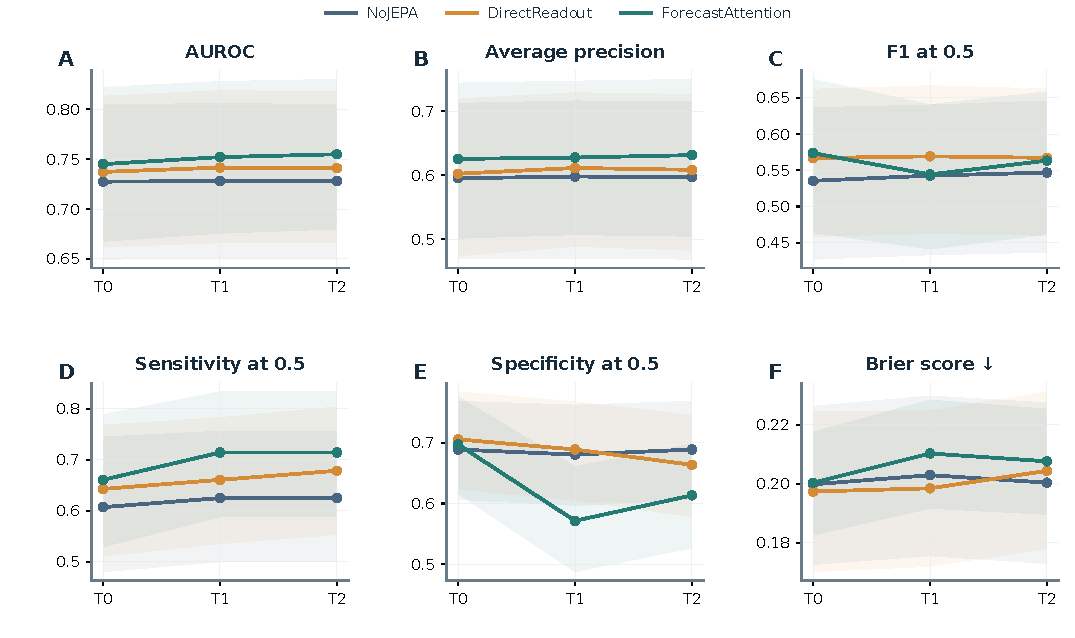
\includegraphics[width=\textwidth]{figures/landmark_performance.pdf}
\caption{Six complementary landmark summaries: AUROC, AP, F1, sensitivity, specificity, and Brier score. All points are calculated from the seed-44 five-fold ensemble probabilities; shading is the conditional 95\% patient-bootstrap interval. The same 175 patients appear at every landmark. A trend in ranking can coexist with a different trend in calibration or error types.}
\label{fig:longitudinal}
\end{figure*}

\begin{figure*}[t]
\centering
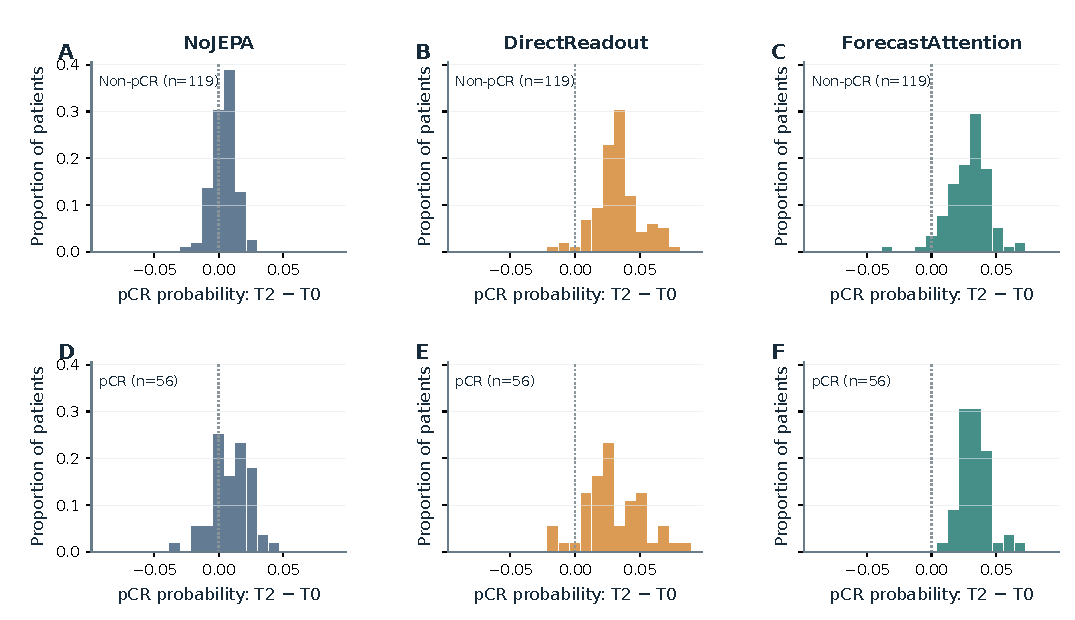
\includegraphics[width=\textwidth]{figures/outcome_score_changes.pdf}
\caption{Outcome-conditioned changes in predicted pCR probability from T0 to T2. Panels separate models and outcome classes. Histograms are calculated directly from the seed-44 five-fold ensemble probability changes for each patient. Changes describe model scores and do not establish an individual treatment effect.}
\label{fig:scorechanges}
\end{figure*}

\section{Supplementary subgroup and training-probe summaries}
\begin{table*}[t]
\centering
\small
\caption{Exploratory subgroup discrimination for the seed44 fivefold probability ensemble. Each patient\textquotesingle s probabilities are averaged over five fold models before computing AUROC; Macro then averages T0--T2 AUROCs. Intervals are paired patient-bootstrap intervals for ForecastAttention minus NoJEPA, conditional on the fitted ensemble. Age 50 is an exploratory reporting cutpoint. Namespace groups are parts of one clinical release, not external cohorts.}
\label{tab:subgroups}
\begin{tabular}{lrrr}
\toprule
Subgroup ($n$/pCR+) & NoJEPA & Full & $\Delta$ AUROC [95\% interval] \\
\midrule
HR+/HER2- (68/11) & 0.687 & 0.716 & +0.029 [-0.032, +0.091] \\
HR+/HER2+ (31/12) & 0.618 & 0.649 & +0.031 [-0.075, +0.132] \\
HR-/HER2+ (14/7) & 0.837 & 0.912 & +0.075 [-0.025, +0.250] \\
HR-/HER2- (62/26) & 0.642 & 0.675 & +0.033 [-0.013, +0.084] \\
Age $<$50 (90/29) & 0.673 & 0.687 & +0.014 [-0.015, +0.042] \\
Age $\geq$50 (85/27) & 0.785 & 0.817 & +0.031 [-0.004, +0.073] \\
ISPY2 namespace (125/39) & 0.680 & 0.702 & +0.022 [-0.008, +0.054] \\
ACRIN-6698 namespace (50/17) & 0.846 & 0.876 & +0.031 [-0.014, +0.082] \\
\bottomrule
\end{tabular}
\end{table*}

\begin{table*}[t]
\centering
\small
\caption{Archived seed44 epoch 20 fixed-training-probe diagnostics. These are descriptive means of five fold-specific skills, distinct from probability ensembling for pCR. Skill is $1-\mathrm{L1}_{forecast}/\mathrm{L1}_{copy}$ within each snapshot\textquotesingle s EMA coordinates; positive is better than holding the landmark state constant. Forecast targets require a continuous actually observed visit chain. These are training-probe summaries, not best-checkpoint holdout forecast evaluations. NoJEPA has no trained-world diagnostic.}
\label{tab:worldprobe}
\begin{tabular}{lrrr}
\toprule
Model & Horizon 1 skill & Horizon 2 skill & Horizon 3 skill \\
\midrule
NoJEPA & -- & -- & -- \\
DirectReadout & +0.026 & +0.050 & +0.193 \\
ForecastAttention & -0.037 & -0.015 & +0.024 \\
\bottomrule
\end{tabular}
\end{table*}


\section{Reproducibility and reporting items to complete}
The source package includes aggregate CSV files, source-report hashes, reproducible metric and figure scripts, the paired DeLong and patient-bootstrap procedures, score-swap sensitivity checks, and the official article class. The main significance CSV includes raw $p$ values, within-family Holm adjustment, and adjustment over all 90 tests as a sensitivity analysis. It contains no patient identifiers, patient-level prediction rows, original MRI volumes, or model checkpoints. The method figure includes only rendered, anonymous development-image slices. Each model uses training seed 44. Five fold probabilities are averaged per patient before computing pCR metrics. Individual-fold metrics are retained only for numerical audit; archived training diagnostics are summarized across fold models in their own latent coordinates.

\todo{Before submission, complete author and ethics statements; verify the precise pCR pathology definition; document codec and segmentation patient-level pretraining provenance; add matched external baselines and a prospectively locked seed-selection policy; audit external-cohort independence; and confirm the journal's current submission and anonymization requirements.}
